\documentclass[aspectratio=169, 10pt]{beamer}

% --- Packages ---
\usepackage[utf8]{inputenc}
\usepackage[T1]{fontenc}
\usepackage{graphicx}
\usepackage{booktabs}
\usepackage{listings}
\usepackage{xcolor}
\usepackage{tikz}
\usepackage{adjustbox}
\usepackage{helvet}
\usepackage{hyperref}

\usetikzlibrary{shapes.geometric, arrows.meta, positioning, calc, fit, backgrounds, decorations.markings}

% --- Texas 2036 Inspired Colors ---
\definecolor{TXBlue}{RGB}{0, 45, 114}
\definecolor{TXRed}{RGB}{191, 13, 62}
\definecolor{TXGray}{RGB}{241, 241, 241}
\definecolor{TXDarkGray}{RGB}{80, 80, 80}
\definecolor{TXOrange}{RGB}{191, 87, 0}
\definecolor{TXOrange_bright}{RGB}{221, 107, 32}
\definecolor{policyorange}{RGB}{232, 97, 41} %more reddish in color

\hypersetup{colorlinks=true,linkcolor=TXBlue,urlcolor=TXBlue}

% --- Beamer Theme Customization ---
\setbeamercolor{palette primary}{bg=TXBlue, fg=white}
\setbeamercolor{palette secondary}{bg=TXOrange_bright, fg=white}
\setbeamercolor{structure}{fg=TXBlue}
\setbeamercolor{titlelike}{parent=palette primary}
\setbeamercolor{frametitle}{bg=TXBlue, fg=white}
\setbeamercolor{section in head/foot}{parent=palette primary}

\setbeamertemplate{navigation symbols}{}
\setbeamertemplate{itemize items}[circle]
\setbeamerfont{frametitle}{series=\bfseries, size=\Large}
\setbeamerfont{title}{series=\bfseries, size=\huge}

% Footer
\setbeamertemplate{footline}{
  \leavevmode%
  \hbox{%
  \begin{beamercolorbox}[wd=.333333\paperwidth,ht=2.25ex,dp=1ex,center]{palette primary}%
    Eric A. Booth (Texas2036.org)
  \end{beamercolorbox}%
  \begin{beamercolorbox}[wd=.333333\paperwidth,ht=2.25ex,dp=1ex,center]{palette primary}%
    PVAMU Workshop 2026
  \end{beamercolorbox}%
  \begin{beamercolorbox}[wd=.333333\paperwidth,ht=2.25ex,dp=1ex,right]{palette primary}%
    \insertframenumber{} / \inserttotalframenumber\hspace*{2ex} 
  \end{beamercolorbox}}%
  \vskip0pt%
}

% Code Style
\lstdefinelanguage{Stata}{
    morekeywords={gen, replace, label, bysort, expand, csdid, estat, plot, graph, export, use, clear, tabulate, estimates, store, esttab, ereturn, matrix, colnames, rownames},
    morecomment=[l]{*},
    morecomment=[l]{//},
    morestring=[b]",
    sensitive=false
}

\lstset{
    language=Stata,
    basicstyle=\ttfamily\scriptsize\color{TXDarkGray},
    keywordstyle=\color{TXBlue}\bfseries,
    commentstyle=\color{gray}\itshape,
    stringstyle=\color{TXRed},
    breaklines=true,
    showstringspaces=false,
    frame=single,
    rulecolor=\color{TXBlue!30}
}

% --- Global TikZ Styles for this Prezi ---

% --- Title Information ---
\title{Applied Policy Evaluation}
\subtitle{{\color{TXOrange}{Implementation Science, AI, and Modern Causal Inference}}}

\author{\textbf{Eric Booth}}
\institute{
    {Senior Researcher, Texas 2036} \\[.25em] \href{https://www.Texas2036.org}{\texttt{www.Texas2036.org}} \\[0.5em]
   % {President, Far Harbor, LLC} // \href{https://www.farharbor.com}{\texttt{www.farharbor.com}} %
	\url{www.github.com/ericabooth}  (slides and materials)
}
\date{May 2026}

% --- Logo Inclusion ---
\titlegraphic{
    \vfill
    
\includegraphics[width=3.5cm]{19_Texas2036_Primary_2Color_fixed.png}
}

\begin{document}
% Slide 1: Title
\begin{frame}[plain] % 'plain' removes the default header/footer for the title slide
    \begin{center}
        \footnotesize
        \color{TXBlue}{\textbf{Prairie View A\&M University - National Science Foundation} \\ 
        Excellence in Research Summer Workshop}
    \end{center}
    
    \vspace{-1em} % Adjust this to pull the title closer if needed
    
    \titlepage
\end{frame}

%slide 1a: Lecture subtitle slide and goals
\begin{frame}{Motivating questions}
    \textbf{\Large\centering{Lecture 1: The Modern Evaluator's Toolkit}}
    \vfill
\begin{enumerate}
\item What does modern policy and program evaluation look like in an applied context?
\item How do we make applied evaluation visible and impactful?
\item How is the evaluator toolkit changing?
\end{enumerate}
\end{frame}

% Slide 3: The Embedded Evaluator
\begin{frame}{Relevant and Impactful Evaluation of Policy and Programs}

%\pause
 \begin{columns}[t]
\begin{column}{0.48\linewidth}
        \begin{itemize}
            \item<1-> Person-centered
            \item<1-> Actionable
            \item<1-> Accessible
            \item<1-> Concise
        \end{itemize}
    \end{column}
    \begin{column}{0.48\linewidth}
        \begin{itemize}
            \item<2-> Transparent
            \item<2-> Supports program scalability
            \item<2-> Promotes sustainabiity
            \item<2-> Modern tool-embracing: outcomes, measurement, ROI
        \end{itemize}
\end{column}
    \end{columns}    
    \end{frame}
    
% Slide 2: Lecture 1 : defining terms
\begin{frame}{Classic evaluation}

\begin{description}
\item[Core principals] Planning, Measurement, Analysis, and Feedback
	\begin{itemize}
	 \item Theory of Change
	 \item Logic Models
	\end{itemize} \pause
\item[Relevance] focused on externalization/generalization "Does this program or intervention work?"
\item[Timing] often post-hoc w/feedback for future implementations and evaluation
\item[Deliverables] classic reports, publications, policy briefs, toolkits or dashboards
\end{description}
 
\end{frame}

\begin{frame}{Emerging, modern evaluation}
It redefines some of those elements \ldots
\vspace{1em}
\begin{description}
\item[Core principles] Contextual mapping, Implementation Fidelity, and Adaptation
	\begin{itemize}
	 \item Implementation Frameworks (e.g., CFIR, RE-AIM)
	 \item Continuous, Iterative Feedback Loops and Improvements
	\end{itemize} \pause
\item[Relevance] focused on context and mechanism: "How and why does this work \textit{here} or for \textit{this group}? Who is left out or falls through the gaps?"
\item[Timing] iterative and real-time; experiments embedded directly into the rollout
\item[Deliverables] active diagnostic engines, adaptation / course-correction logs, gap analyses, quantification of uncertainty (\color{TXOrange}{\textit{Trustworthiness of results}})
\end{description}
\pause
\vfill
\begin{quote} \centering \color{TXOrange}{Applied evaluation is no longer just an external, 3rd party audit... \\ it is a strategic partnership in the implementation lifecycle.} \end{quote}  
\end{frame}



% Slide 4: IS Frameworks
\begin{frame}[fragile]{Implementation Science in Practice}
 \begin{center}
 \color{TXOrange}{  If clinical or policy research asks: }
  \begin{quote}"Does this intervention improve outcomes in a controlled environment?" (Effectiveness, Causality) \end{quote}
  \color{TXOrange}{  Implementation Science asks: }
 \begin{quote}"Why do evidence-based practices frequently fail to reach their full potential in real-world settings, and how do we systematically bridge that gap?"  \end{quote}
\end{center}
   Frameworks:
    \begin{itemize}
      \item \textbf{RE-AIM playbook:} Reach, Effectiveness, Adoption, Implementation,    Maintenance.
      	\item \textbf{Consolidated Framework for Implementation Research (CFIR):}    Consideration of site characteristics to explain \textit{why} things work in specific    settings; work iteratively with practitioners to understand complex environment and     implementation.
    \end{itemize}
   
\textsf{  \hfill   \color{TXOrange}{ \ldots  Why does this matter?}} 

\end{frame}

% Slide 4a: IS Frameworks
\begin{frame}[fragile]{Implementation Science in Practice: Why Important?}

{\color{TXOrange}{\textsf{tl;dr}}} IS transforms evaluation \textit{from a "passive report-card" at the end of a grant cycle} into an \textbf{active diagnostic engine that provides real-time data to help} program funders, nonprofit leaders, and state agencies course-correct in real-time.\\ \pause
\hrulefill
\vfill
\footnotesize
\begin{description}
    \item[\textbf{\textcolor{TXBlue}{Evidence is not self-executing:}}]A policy that works in a controlled pilot often fails when scaled. IS provides the empirical tools to measure \textit{why}\ldots locating the exact friction in leadership buy-in, incentives, or frontline capacity.    
    \item[\textbf{\textcolor{TXBlue}{Context is a feature, not a bug:}}]Classical evaluation controls for the "setting" as noise; IS investigates the setting (both inner organizational capacity and outer political environment) as a possible driver of success.    
    \item[\textbf{\textcolor{TXBlue}{Closing the ``Know-Do'' Gap:}}] moves beyond outcome measurement to provide a rigorous approach : \pause
    \begin{itemize}
        \item \textbf{Fidelity Monitoring:} Distinguishing between \textit{program failure} (bad idea) and \textit{implementation failure} (bad execution).
        \item \textbf{Systematic Adaptation:} Modifying a policy for local needs without losing its core ``active ingredients.''
        \item \textbf{{Scale \& Sustain:}} Planning for permanent integration from Day 1, rather than just surviving a pilot grant cycle.
    \end{itemize}
 \end{description}

\end{frame}

% Slide 5: AI Workflows
\begin{frame}[fragile]{How is the evaluator toolkit changing?}

\textbf{Tried and true}: Theory, planning/logic, high-impact communications, data-driven \\
\textbf{New and emerging}: AI as a (trained) Thought Partner and Blindspot Detector \\ \vfill
\pause
\begin{quote} In Data Analysis we try to avoid {\color{TXOrange}{``Garbage In / Garbage Out"}} \\ \pause
 \ldots \ldots \ldots With AI we try to detect \color{TXOrange}{``Garbage In / Gospel Out"} \end{quote}
 \pause
    \textbf{The AI Sieve Strategy:}
    \begin{enumerate}
        \item Human-centered, textured, deliberative, and raw inputs - discuss and direct AI as you would with a coauthor or Research Assistant \pause
        \item Train AI on past work and archival documents
        \item Train Agents to check for bias, blindspots, POV of various audiences/cultures \pause
        \item Run AI against other models/LLMs to ask for issues and uncertainty; \\ \textsf{What did the other AI LLMs miss or mistake?}
        \item Then read, edit, and rewrite to ensure the human fingerprint \pause
        \item {\color{TXBlue}{Gut-check and scrutinize}} the work with trusted stakeholders and experts.  \\
        Evaluation and research as a profession is about \\ taking responsibility for the truth.             \end{enumerate} 
    \begin{tikzpicture}[remember picture, overlay]
    \node [shift={(-2cm, 1.33cm)}, rotate=2] at (current page.south east)
        { 
\includegraphics[scale=0.33]{eye.jpeg} };
\end{tikzpicture}
% \hfill
\includegraphics[width=0.12\textwidth]{eye.jpeg}
    \vfill 
    \end{frame}

\begin{frame}[fragile]{How is the evaluator toolkit changing?}

{\color{TXBlue}{ \textit{AI cannot squint \pause \\ \hspace{2em}\ldots and it lacks skin in the game.} \pause \\ \hspace{4em} \ldots when a model hallucinates, it doesn't lose a job or funding; you do. }} \\[2em]
\pause

    \centering
 {  \color{TXRed}{ \textbf{\large Consider: How do we embrace AI while avoiding reputational and quality issues?}} }\\
  \flushleft
\vfill  \pause 
\textbf{ Embracing AI can certainly be:} \\ \hspace{.38em} (1)  efficient (2)  evidence of being a custodian of funder or public dollars \\ \hspace{.38em}  (3)  higher quality  (4) a democratizer of sophisticated / expensive methods or tools.\\[1.25em]
  
  \underline{Apparent }AI content, especially when it lacks substance or accuracy, may alienate your funders, stakeholders, and audiences. \textit{IS may magnify this risk} \\[1em]
  \pause
  \hfill \ldots When audiences lose trust - it's difficult to earn it back. \\[1em]

\end{frame}


%  Data, Analysis, and AI 
\begin{frame}{Data, Analysis, and AI \\ \small(roadmap for next session this afternoon)}
    \begin{itemize}
        \item \textbf{Questions in focus:} Example: Loss of medicaid coverage at 60 days postpartum.
        \item \textbf{Connections to data:} ICPSR, Accessing APIs 
        \item \textbf{Analysis in realtime:} Stata and R as core tools; open-science framework
        \item \textbf{Leveraging AI strategically:} Productization ; Non-transparent/non-reproducible but useful none-the-less; check for error and blindspots
        \item \textbf{Results that matter:} Clarity earns attention; attention enables impact 
 
    \end{itemize}

\end{frame}


%  Data, Analysis, and AI 
\begin{frame}{Data, Analysis, and AI \\ Results that matter}
\begin{quote}The choice in the analysis toolkit is not between binary trade-offs: descriptive vs. inferential, summary vs. causal, formative vs. predictive, etc \end{quote}  
\vfill
 \textbf{Tell stories with analyses that: }
\pause 
    \begin{itemize} 
	\item {\color{TXOrange} Zoom out: }Summarize and tell the story for the outcome of interest
	\begin{itemize}
	   \item {\color{TXOrange}Find the lever: }Pick outcomes that can be augmented! 
	  \item Inspection by sub-population or time period of interest (e.g. cross-tabulations) \pause
	\end{itemize}
		\item {\color{TXOrange} Dig deeper: }consider unpacking patterns that match real world complexity or explore 'what if' scenarios
	\item {\color{TXOrange} Zoom in: }vignettes of \textit{common stories/profiles} of study population
 
    \end{itemize}

\end{frame}





%%%%%%%%%%%%%%%%%%%%%%%%%%%%%%%%%%%%%%%%%%%%
%  Lecture 2 Overview
\begin{frame}{Lecture 2: From Archive to Action}
    \textbf{Technical Walkthrough: Medicaid Expansion \& PRAMS}
    \vfill
    \begin{itemize}
        \item Sourcing Data from ICPSR (study \#114516)
        \item The "Postpartum Cliff" Policy Shock.
        \item Staggered Adoption \& A Causal Story.
        \item Policy tool: Difference-in-Difference analysis (via Stata \texttt{csdid})
        \item 3 Hands-on examples in Stata \& R
    \end{itemize}
\end{frame}

\begin{frame}{Sourcing data from ICPSR (and elsewhere)}
    \textbf{Key tools to consider}
    \vfill
    \begin{itemize}
        \item Data accessible via API (automate download, updates when new data come out)
        \item Use AI to access and clean/harmonize data (but use cross-checks for data integrity!)
        \item Carefully check codebooks for recoding, weighting, or data inclusion rules (gut check with experts or existing literature)
    \end{itemize}
\end{frame}


% The Scenario
\begin{frame}{Scenario: The Postpartum Cliff}
    \begin{itemize}
        \item \textbf{Policy:} ACA Medicaid Expansion (Continuous Coverage).
        \item \textbf{The Problem:} Loss of coverage at 60 days postpartum.
    \end{itemize}
    \vfill
    \centering
    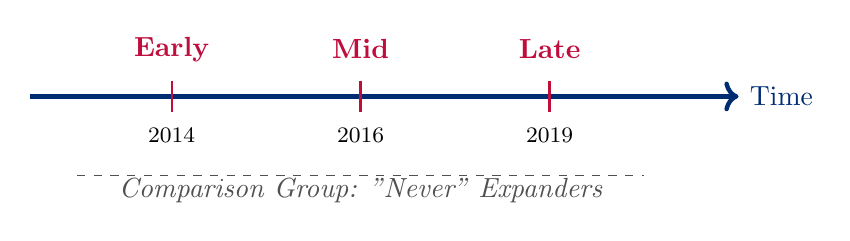
\begin{tikzpicture}[xscale=1.2]
        % Timeline
        \draw[->, ultra thick, TXBlue] (-0.5,0) -- (7,0) node[right]{Time};
        
        % Events
        \foreach \x/\year in {1/2014, 3/2016, 5/2019} {
            \draw[thick, TXRed] (\x, 0.2) -- (\x, -0.2);
            \node at (\x, -0.5) {\footnotesize \year};
        }
        
        % Labels
        \node[TXRed, font=\bfseries] at (1, 0.6) {Early};
        \node[TXRed, font=\bfseries] at (3, 0.6) {Mid};
        \node[TXRed, font=\bfseries] at (5, 0.6) {Late};
        
        \node[TXDarkGray, font=\itshape] at (3, -1.2) {Comparison Group: "Never" Expanders};
        \draw[dashed, TXDarkGray] (0,-1) -- (6,-1);
    \end{tikzpicture}
\end{frame}

% Baseline Data
\begin{frame}{The Context: Baseline Characteristics (2010)}
    \centering
    \begin{tabular}{lccc}
\toprule
& 2010 Avg & 2020 Avg & Diff \\
\midrule
Postpartum Insurance Rate & 64.7 & 78.0 & +13.3\% \\
Postpartum Depression Rate & 19.8 & 15.3 &  -4.5\% \\
\bottomrule
\end{tabular}

    \vfill
    \footnotesize \textit{Issue: doesnt account for complexity of the roll-in of the ``treatment" policy intervention across time and states}
\end{frame}

%scatter figure
\begin{frame}{Data exploration}
    \centering
    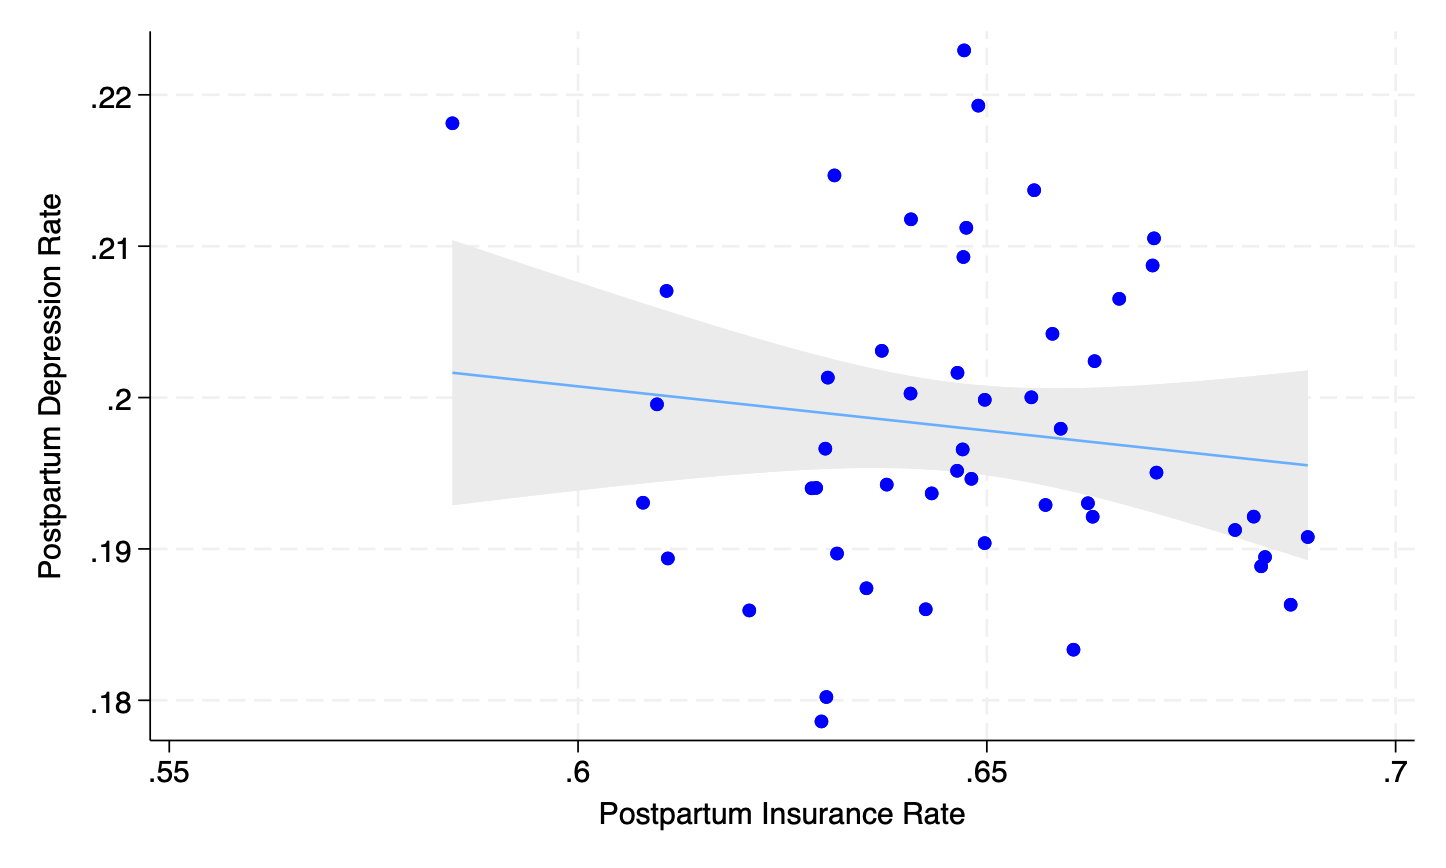
\includegraphics[width=0.95\textwidth]{../scripts/fig0.png}
\end{frame}


%descriptive figure
\begin{frame}{Data exploration}
    \centering
    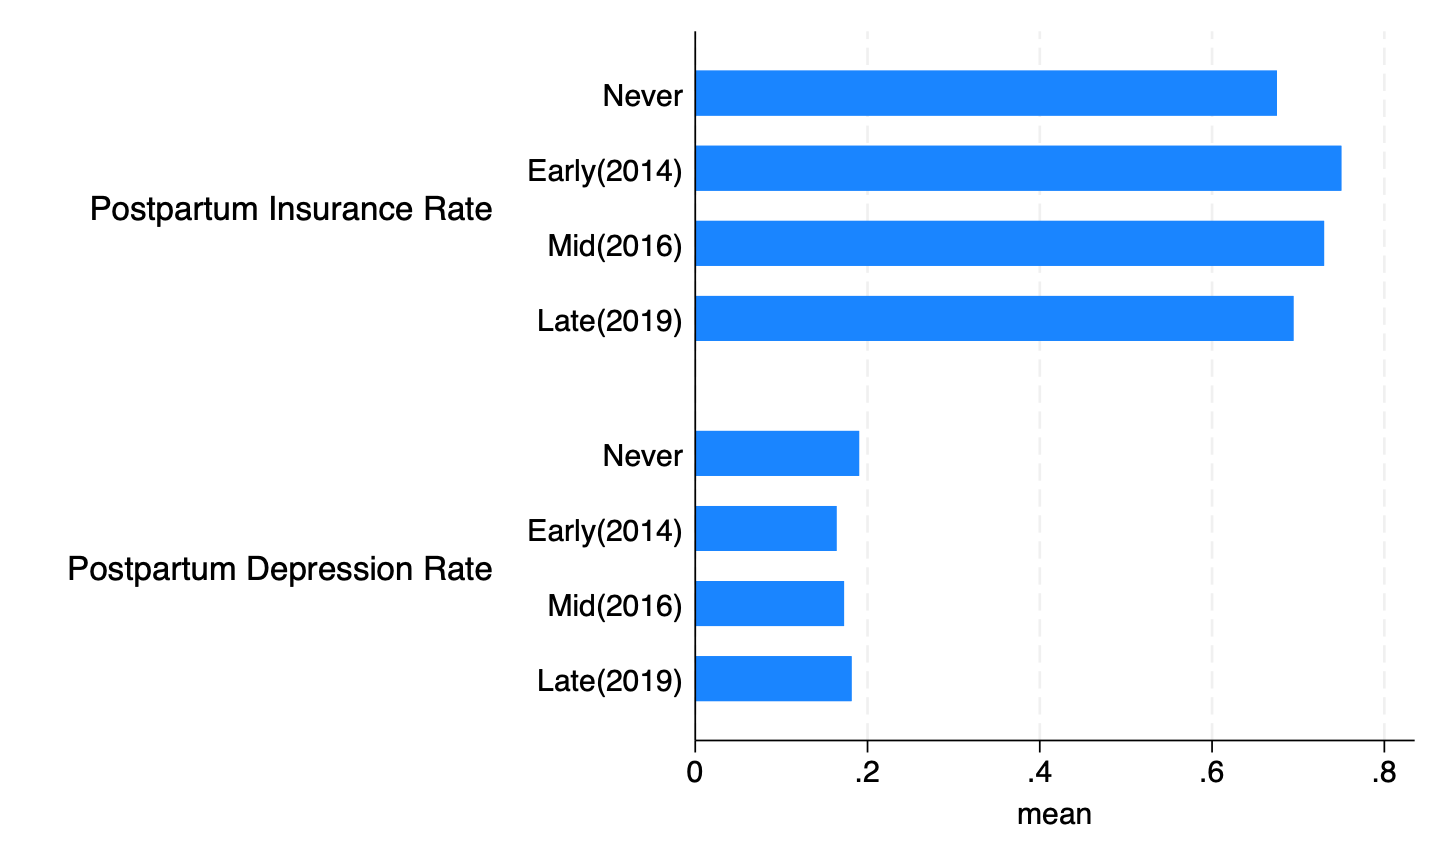
\includegraphics[width=0.95\textwidth]{../scripts/fig1.png}
\end{frame}


%descriptive figure
\begin{frame}{Data exploration}
    \centering
    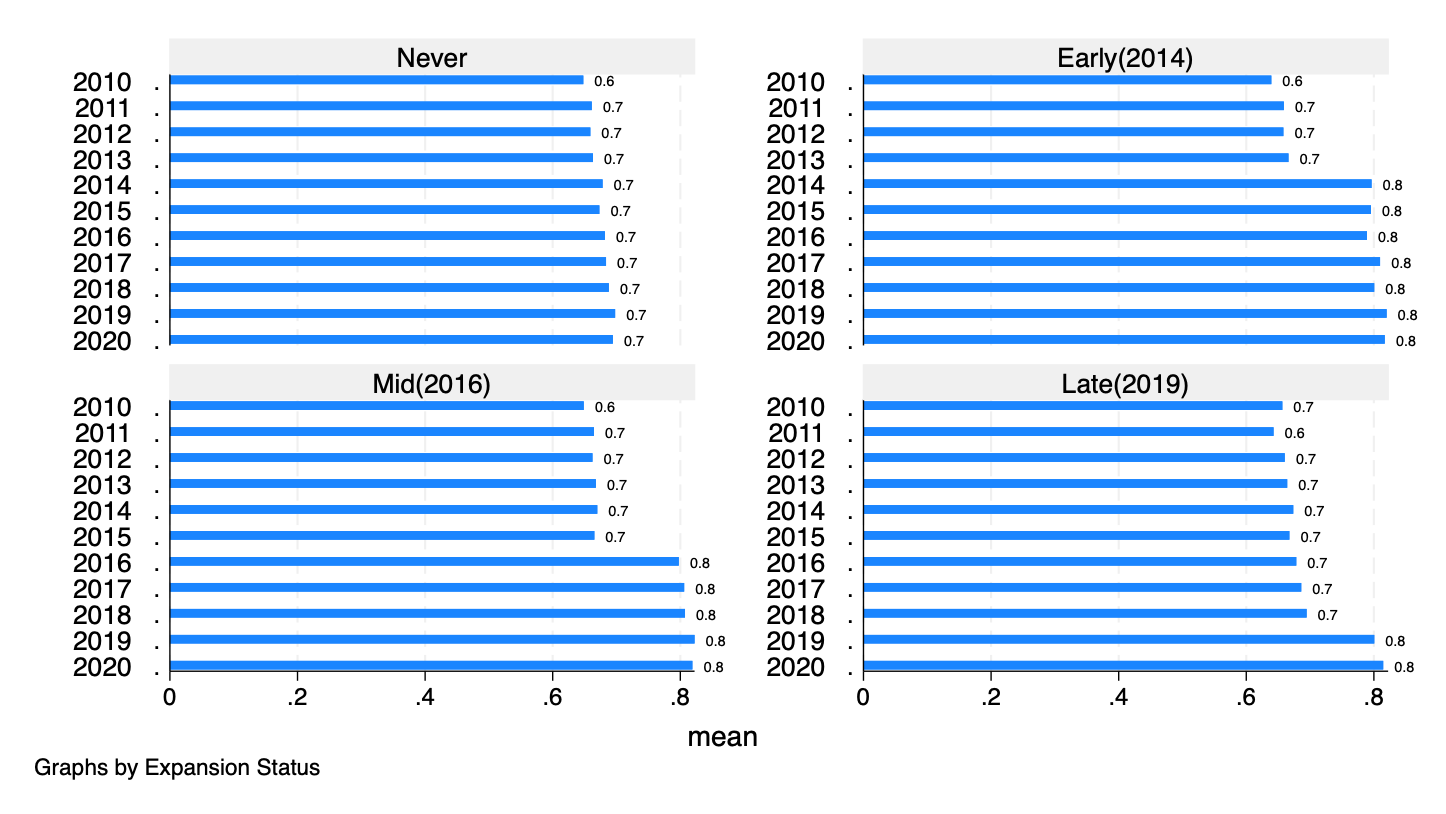
\includegraphics[width=0.95\textwidth]{../scripts/fig2.png}
\end{frame}



%DID figure
\begin{frame}{Detecting changes before and after an intervention}
We compare how much outcomes changed over time in states that adopted the policy versus not;  \textbf{the difference between those two changes} is our {\color{TXOrange}{intervention effect}} \pause
    \centering
    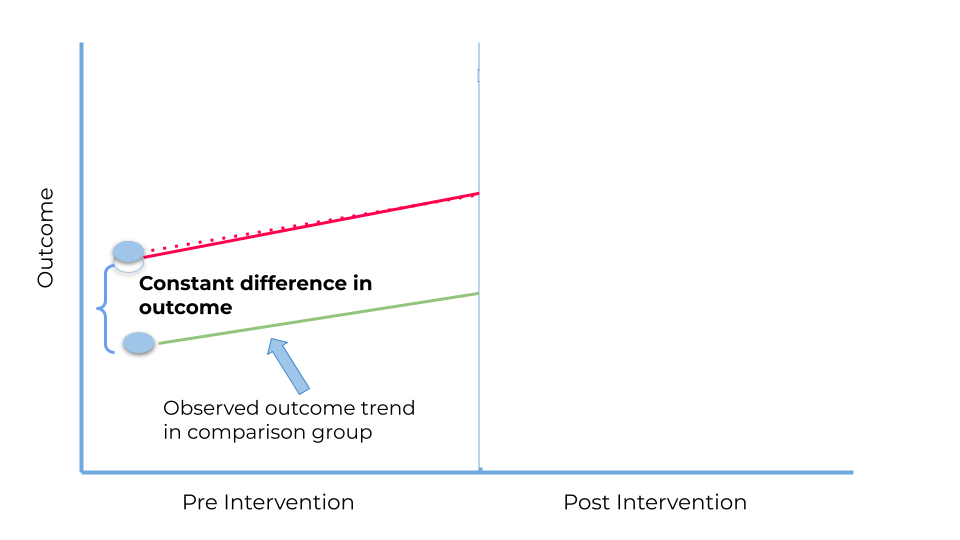
\includegraphics[width=0.90\textwidth]{../figures/did.png}
\end{frame}


%DID figure
\begin{frame}{Detecting changes before and after an intervention}
We compare how much outcomes changed over time in states that adopted the policy versus not;  \textbf{the difference between those two changes} is our {\color{TXOrange}{intervention effect}} 
    \centering
    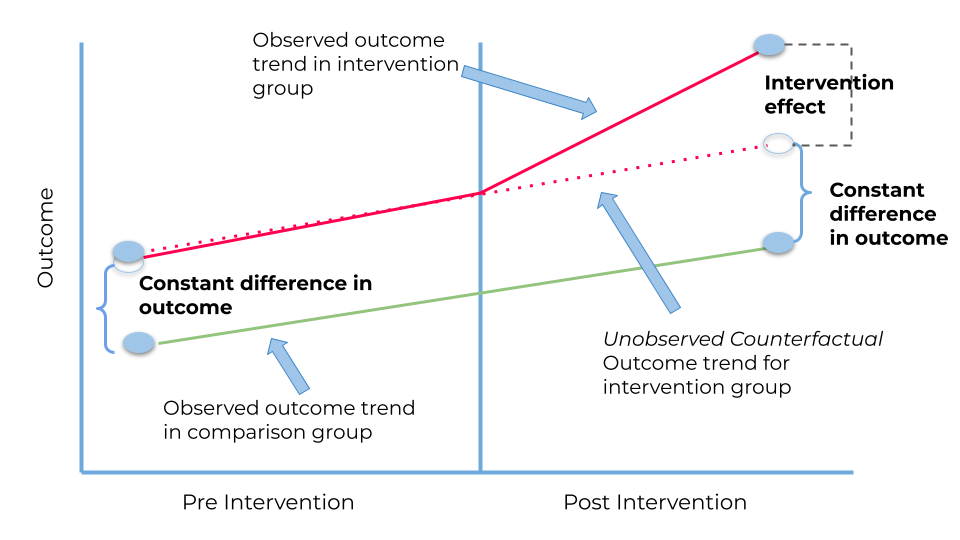
\includegraphics[width=0.90\textwidth]{../figures/did2.png}
\end{frame}




% The Solution (csdid)
\begin{frame}[fragile]{Implementing Modern DiD}
    \textbf{Stata Command:} \texttt{csdid}
    \vfill

    \begin{itemize}
        \item \textbf{ivar:} Panel ID (State).
        \item \textbf{tvar:} Time variable (Year).
        \item \textbf{gvar:} Treatment group (Year of expansion, 0 if never).
    \end{itemize}
    \vfill
    \begin{lstlisting}[basicstyle=\normalsize\ttfamily]
//  DID Aggregate Effects
csdid insured_rate, ivar(state) time(year) gvar(gvar)  

  // Simple average
     estat simple
 // Group-time average
    estat group

// Diff-in-Diff Study Visual
csdid_plot
    \end{lstlisting}
\end{frame}

% Slide 13: Results (Visual)
\begin{frame}{The Picture: Event Study Plots}
    \centering
    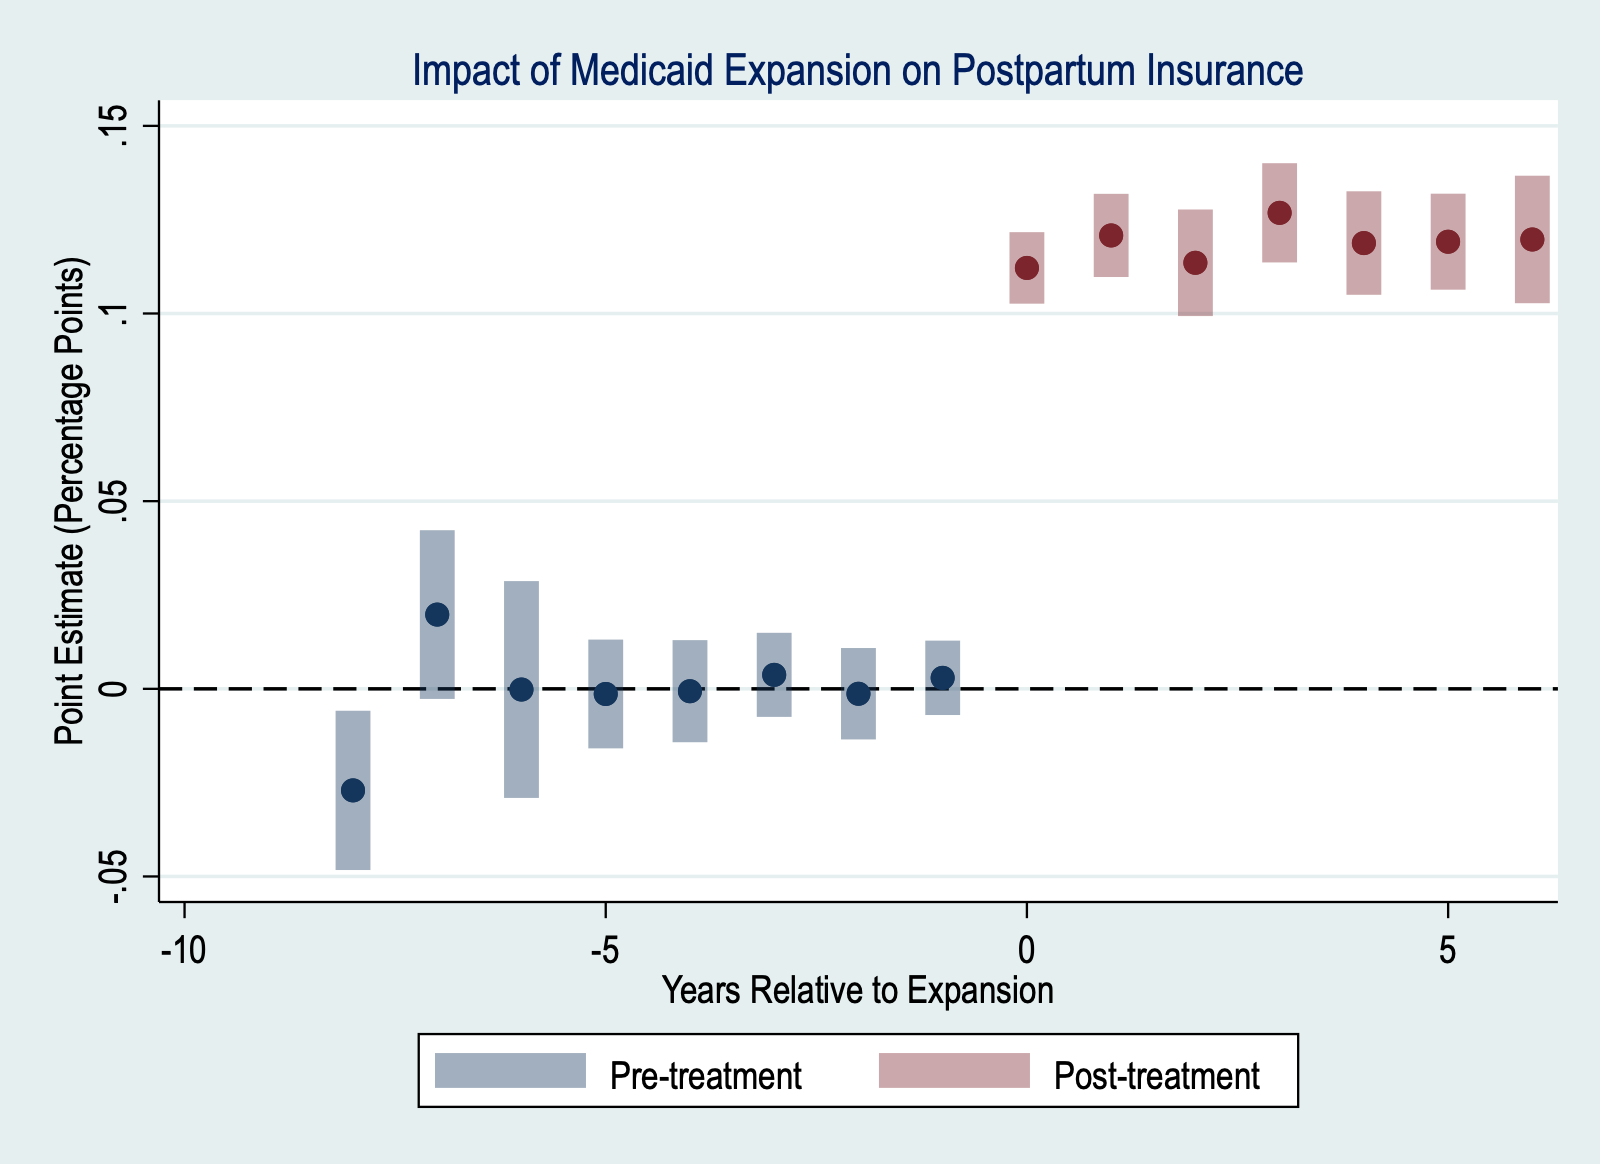
\includegraphics[width=0.65\textwidth]{../figures/event_study_insurance.png}
    \vfill
    \raggedright
    \footnotesize \textit{No upward Pre-treatment trend; Post-treatment sustained post-treatment boost. \\ Each cohort shows a large, immediate, and sustained jump in postpartum insurance rates in the year of expansion}
\end{frame}

% Slide 14: Results (Table)
\begin{frame}{The Table: Aggregated / Adjusted Effects}
    \centering
    \begin{tabular}{lc}
\toprule
\textbf{Outcome: Insurance Rate} & \textbf{Estimate} \\
\midrule
Aggregate ATT & 0.118*** \\
& (0.004) \\
\bottomrule
\end{tabular}

    \vfill
    \raggedright
     \textit{Aggregated Simple Average Effect Size (ATT) across all groups
    and times. Aggregate ATT = $+$11.8 percentage points (SE=0.004, z=28.16,
    $p < 0.001$, 95\% CI: 11.0--12.7 pp). }\\
\vfill 
  Group-level averages are tightly clustered (10.5 --12.9 pp),  indicating consistent effects regardless of when a state expanded.

% | Cohort | Year of jump | ATT at expansion | Still sustained by 2020 |
% |---|---|---|---|
% | G2014 | 2013→2014 | +11.5 pp (p<0.001) | ~+12.0 pp |
% | G2016 | 2015→2016 | +12.4 pp (p<0.001) | ~+13.3 pp |
% | G2019 | 2018→2019 | +9.6 pp (p<0.001) | ~+11.4 pp |
\end{frame}





\begin{frame}{Synthesis: \\
Detecting the "So What?" using AI as a thought partner}
\begin{description}
    \item[\textcolor{TXBlue}{Translate the model:}]  Package estimates in plain language and visualizations for three audiences: a state legislator, a frontline caseworker, and an affected mother. \textbf{Where the stories diverge, you may have a policy lever.} \pause

    \item[\textcolor{TXBlue}{Surface the knowledge gap:}] AI can help unpack where insurance gain \textit{should} produce downstream — birth outcomes, ER utilization, mental health — then flag where your data cannot yet follow. \textbf{That gap is your next research question.} \pause

    \item[\textcolor{TXBlue}{Stress-test your story:}] Run your AI Sieve \& ask: \textit{"What would a skeptical funder object to?" etc. } (\textbf{Pre-empting rival explanations}) \pause

    \item[\textcolor{TXBlue}{Check for hidden populations:}] Prompt AI to ask who is \textit{absent} from the data — undocumented mothers, rural non-responders, language minorities \ldots \textbf{Silence in the data is itself a finding.} \pause

    \item[\textcolor{TXBlue}{Preserve the human fingerprint:}] AI drafts the frame; you supply the texture. Rewrite: \textbf{anchor to authentic vignette or stakeholder experience.}
\end{description}
\end{frame}

% hands on activities
\begin{frame}[fragile]{Hands on: Walk through of a few Stata \& R examples using ICPSR datasets}
\begin{enumerate}
\item Medicaid expansion example \& dashboard visualization \pause
\item 
Pregnancy Risk Assessment Monitoring System (PRAMS) MCH Indicators 2016-2022 (ICPSR \#221043) \pause
\item TX STAAR performance before/after test redesign in Spring 2023 (Using API \& AI to download and merge together data overtime) from Dell Foundation funded \url{Zelma.ai}
\end{enumerate}
\end{frame}


% Slide 16: Conclusion
\begin{frame}[plain]
    \centering
    \huge \color{TXBlue} \textbf{Questions?}
    \vfill
    \large Eric A. Booth \\ [.5em] Texas 2036.org \\[1em]
    \footnotesize eric.a.booth@gmail.com \\
	\url{www.github.com/ericabooth}
\end{frame}

\end{document}
